\section{UClient Class Reference}
\label{classUClient}\index{UClient@{UClient}}
Linux implementation of {\bf UAbstract\-Client}{\rm (p.\,\pageref{classUAbstractClient})}.  


{\tt \#include $<$uclient.h$>$}

Inheritance diagram for UClient::\begin{figure}[H]
\begin{center}
\leavevmode
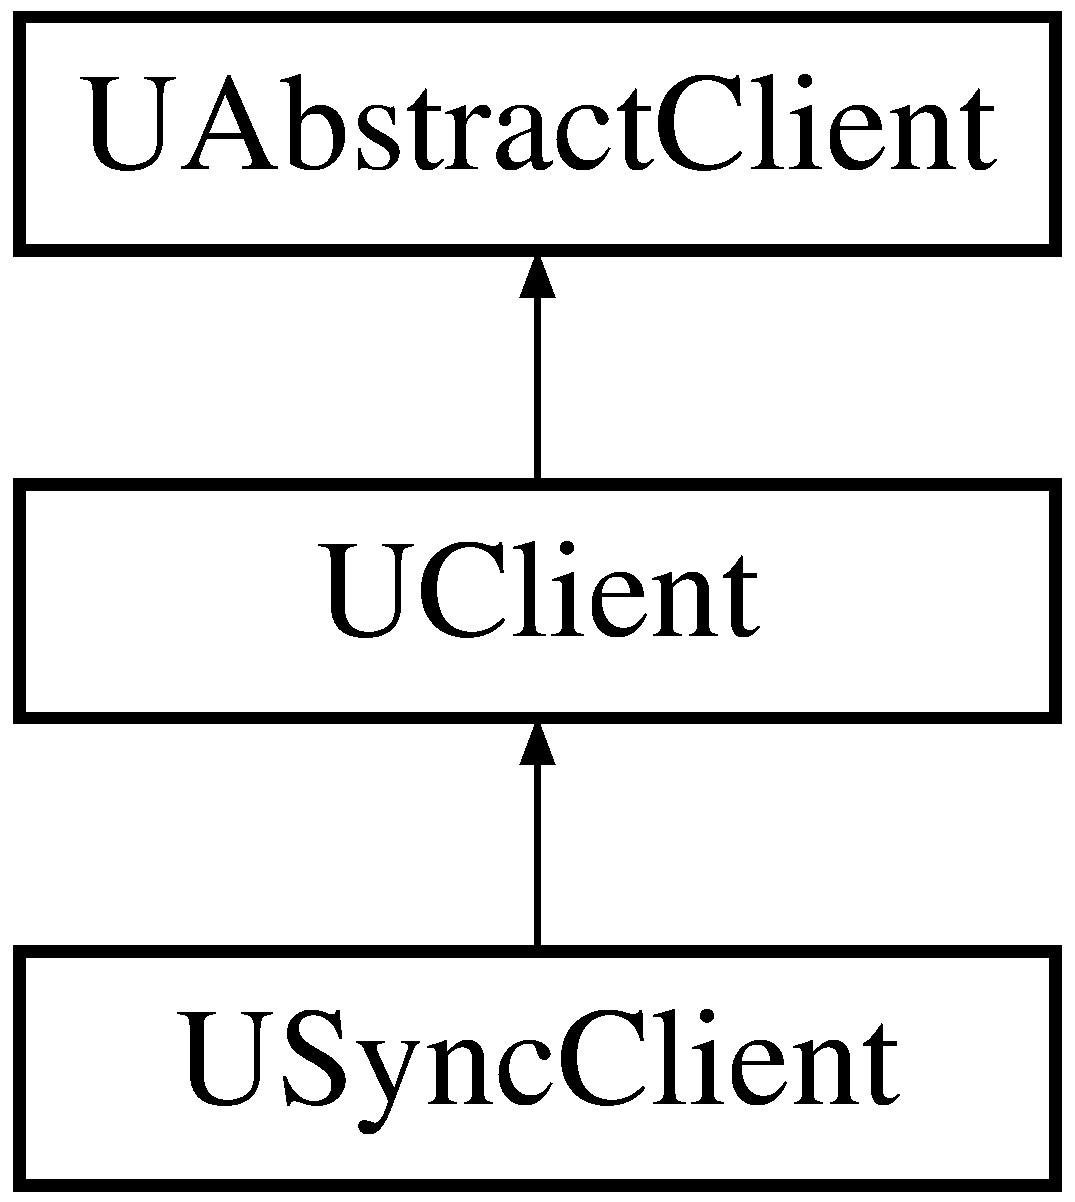
\includegraphics[height=3cm]{classUClient}
\end{center}
\end{figure}
\subsection*{Public Member Functions}
\begin{CompactItemize}
\item 
{\bf UClient} (const char $\ast$\_\-host, int \_\-port={\bf URBI\_\-PORT}, int \_\-buflen={\bf URBI\_\-BUFLEN})
\item 
void {\bf start} ()\label{classUClient_a2}

\begin{CompactList}\small\item\em For compatibility with older versions of the library. \item\end{CompactList}\item 
void {\bf listen\-Thread} ()\label{classUClient_a3}

\begin{CompactList}\small\item\em For internal use. \item\end{CompactList}\item 
virtual void {\bf printf} (const char $\ast$format,...)\label{classUClient_a4}

\begin{CompactList}\small\item\em Notify of an error. \item\end{CompactList}\item 
virtual unsigned int {\bf get\-Current\-Time} ()\label{classUClient_a5}

\begin{CompactList}\small\item\em Get time in milliseconds since an unspecified but constant reference time. \item\end{CompactList}\item 
virtual void {\bf lock\-Send} ()\label{classUClient_a6}

\begin{CompactList}\small\item\em Lock the send buffer for exclusive use by the current thread. \item\end{CompactList}\item 
virtual void {\bf unlock\-Send} ()\label{classUClient_a7}

\begin{CompactList}\small\item\em Unlock the send buffer. \item\end{CompactList}\end{CompactItemize}
\subsection*{Protected Member Functions}
\begin{CompactItemize}
\item 
virtual int {\bf effective\-Send} (const void $\ast$buffer, int size)\label{classUClient_b0}

\begin{CompactList}\small\item\em Queue data for sending, returns zero on success, nonzero on failure. \item\end{CompactList}\item 
virtual bool {\bf can\-Send} (int size)\label{classUClient_b1}

\begin{CompactList}\small\item\em Check if successive {\bf effective\-Send()}{\rm (p.\,\pageref{classUClient_b0})} of cumulated size 'size' will succeed. \item\end{CompactList}\item 
virtual void {\bf lock\-List} ()\label{classUClient_b2}

\begin{CompactList}\small\item\em Lock receive and send portions of the code. \item\end{CompactList}\item 
virtual void {\bf unlock\-List} ()\label{classUClient_b3}

\begin{CompactList}\small\item\em Unlock receive and send portions of the code. \item\end{CompactList}\end{CompactItemize}
\subsection*{Protected Attributes}
\begin{CompactItemize}
\item 
int {\bf sd}\label{classUClient_p0}

\begin{CompactList}\small\item\em Socket file descriptor. \item\end{CompactList}\end{CompactItemize}


\subsection{Detailed Description}
Linux implementation of {\bf UAbstract\-Client}{\rm (p.\,\pageref{classUAbstractClient})}. 

This implementation creates a thread for each instance of UClient, which listens on the associated socket. 



Definition at line 37 of file uclient.h.

\subsection{Constructor \& Destructor Documentation}
\index{UClient@{UClient}!UClient@{UClient}}
\index{UClient@{UClient}!UClient@{UClient}}
\subsubsection{\setlength{\rightskip}{0pt plus 5cm}UClient::UClient (const char $\ast$ {\em \_\-host}, int {\em \_\-port} = {\tt {\bf URBI\_\-PORT}}, int {\em \_\-buflen} = {\tt {\bf URBI\_\-BUFLEN}})}\label{classUClient_a0}


Establish the connection with the server. Spawn a new thread that will listen to the socket, parse the incoming URBI messages, and notify the appropriate callbacks. 

Definition at line 51 of file uclient.cpp.

References urbi::connect(), printf(), and sd.

The documentation for this class was generated from the following files:\begin{CompactItemize}
\item 
{\bf uclient.h}\item 
{\bf uclient.cpp}\end{CompactItemize}
